\chapter{Appendices}

\section{Code and Data Availability}
\label{sec:code-and-data-availability}

Code is available from:

\begin{itemize}
    \item \url{https://github.com/dan-432/DarwinsRNAHunt} contains the positive control and discovery snakemake pipelines and associated analyses.
    \item \url{https://github.com/dan-432/cm-iterative-expansion} contains the logic for and analysis of the itertive expansion of candidate \ac{CM}s.
    \item \url{https://github.com/dan-432/cm-simile} contains the logic for and analysis of the pairwise similarity scoring of candidate \ac{CM}s
\end{itemize}

See top-level README files for further documentation on file structure and running instructions.

Data and computed results are available from \dots

[link to zenodo]

\section{Supplimentary Tables}

\begingroup
\footnotesize
\begin{longtable}{p{0.14\textwidth}p{0.50\textwidth}}
\caption[Positive controls (RNA $\rightarrow$ protein)]{Rfam families used as positive controls for the RNA-to-protein direction.}
\label{tab:positive_controls_input} \\
\hline
Rfam ID & Description \\
\hline
\endfirsthead
\multicolumn{2}{c}{\tablename\ \thetable{} -- continued} \\
\hline
Rfam ID & Description \\
\hline
\endhead
\hline
\multicolumn{2}{r}{\emph{Continued on next page}} \\
\endfoot
\hline
\endlastfoot
RF01315 & CRISPR RNA direct repeat element \\
RF00050 & FMN riboswitch \\
RF00162 & SAM riboswitch \\
RF01734 & Fluoride riboswitch \\
\end{longtable}
\endgroup

\begin{table}[H]
\centering
\caption[Filtering thresholds used in the computational discovery pipeline]{\textbf{Filtering thresholds used in the computational discovery pipeline.}
    The discovery pipeline was run with these filtering thresholds to identify candidate structured RNA elements associated with the \ac{BLUF} protein domain.
    These thresholds were guided by poitive and negative control experiments.}
\label{tab:thresholds}
\begin{tabular}{@{}lll@{}}
\toprule
Step & Parameter & Value \\
\midrule
3.1 Domain search & hmmsearch E-value & $\leq 10^{-5}$ \\
3.2 Flanking extraction & Minimum length & 20\,nt \\
 & Overlap into coding sequence & 5\,nt \\
3.3 Clustering & mmseqs2 minimum sequence identity & 0.4 \\
 & Coverage (mode 3) & $\geq 0.5$ \\
 & Minimum cluster size & 5 \\
 & Trimming padding & 15\,nt \\
3.5 Covariance analysis & R-scape E-value (at least one covarying pair) & $\leq 0.05$ \\
3.6 Calibration & Random sequence length & $0.8$ megabases \\
\bottomrule
\end{tabular}
\end{table}

\begingroup
\footnotesize
\begin{longtable}{p{0.14\textwidth}p{0.36\textwidth}p{0.24\textwidth}p{0.17\textwidth}}
\caption[Discovery pipeline inputs (protein $\rightarrow$ RNA)]{\textbf{Inputs to the protein-to-RNA discovery pipeline}: protein domain (or protein cluster), description, and the GTDB bacterial clade searched. Genomes were filtered at 99.9\% completeness and $\le$1\% contamination for every pair.}
\label{tab:discovery_inputs} \\
\hline
Domain ID & Description & Bacterial taxon (GTDB node) & Role \\
\hline
\endfirsthead
\multicolumn{4}{c}{\tablename\ \thetable{} -- continued} \\
\hline
Domain ID & Description & Bacterial taxon (GTDB node) & Role \\
\hline
\endhead
\hline
\multicolumn{4}{r}{\emph{Continued on next page}} \\
\endfoot
\hline
\endlastfoot
IPR005594 & SecY domain & \emph{f\_\_Burkholderiaceae\_C} (36.0) & Negative control \\
IPR002208 & YadA-like membrane anchor domain & \emph{f\_\_Burkholderiaceae\_C} (36.0) & Negative control \\
IPR021309 & YgaP-like transmembrane domain & \emph{f\_\_Burkholderiaceae\_C} (36.0) & Negative control \\
IPR001029 & Bacterial flagellin N-terminal helical region & \emph{f\_\_Burkholderiaceae\_C} (36.0) & Initially as negative control \\
IPR007024 & BLUF domain & \emph{f\_\_Burkholderiaceae\_C} (36.0) & Test target \\
cluster\_1341 & FMN riboswitch control (protein cluster) & \emph{f\_\_Microbacteriaceae} (100) & Positive control \\
CRISPR\_Cas2 & CRISPR RNA direct repeat element control (Cas2) & \emph{o\_\_Lactobacillales} (92.0) & Positive control \\
\end{longtable}
\endgroup


\begingroup
\scriptsize
\setlength{\tabcolsep}{2pt}
\begin{longtable}{lrrrlrrrrrrr}
\caption[Positive control run clusters (full)]{Top 10 clusters by genome spread for each RNA family.}
\label{tab:cluster_appendix} \\
\hline
Cluster & Genomes & Seqs & Prev. & Position & Up. & Cont. & Strand & Interg. & Purity \\
\hline
\endfirsthead

\multicolumn{12}{c}{\tablename\ \thetable{} -- continued} \\
\hline
Cluster & Genomes & Seqs & Prev. & Position & Up. & Cont. & Strand & Interg. & Purity \\
\hline
\endhead

\hline
\multicolumn{12}{r}{\emph{Continued on next page}} \\
\endfoot

\hline
\endlastfoot

\multicolumn{12}{l}{\textbf{FMN riboswitch (RF00050)}: 1599 clusters, 2009 genomes, 1115 singleton-genome clusters} \\
\hline
204$^\dagger$ & 926 & 934 & 0.4609 & Up 1 & 0.913 & 0.007 & 1.0 & 0.979 & 0.4609 \\
695 & 578 & 748 & 0.2877 & Up 1 & 0.999 & 0.003 & 1.0 & 0.979 & 0.288 \\
600 & 409 & 417 & 0.2036 & Up 1 & 1.0 & 0.01 & 1.0 & 0.981 & 0.3223 \\
89 & 295 & 295 & 0.1468 & Up 1 & 1.0 & 0.01 & 1.0 & 0.98 & 0.147 \\
58 & 189 & 189 & 0.0941 & Down 1 & 0.0 & 0.0 & 1.0 & 0.979 & 0.1547 \\
340 & 188 & 188 & 0.0936 & Up 1 & 1.0 & 0.005 & 1.0 & 0.973 & 0.2709 \\
1453 & 119 & 119 & 0.0592 & Down 2 & 0.0 & 0.0 & 1.0 & 0.975 & 0.1941 \\
100 & 96 & 99 & 0.0478 & Down 1 & 0.111 & 0.0 & 0.869 & 1.0 & 0.0478 \\
1501 & 90 & 93 & 0.0448 & Down 1 & 0.462 & 0.0 & 0.72 & 0.935 & 0.0448 \\
113 & 71 & 71 & 0.0353 & Up 1 & 1.0 & 0.0 & 0.0 & 0.958 & 0.7474 \\
\hline

\multicolumn{12}{l}{\textbf{SAM riboswitch (RF00162)}: 2247 clusters, 1535 genomes, 1553 singleton-genome clusters} \\
\hline
831$^\dagger$ & 634 & 873 & 0.413 & Up 1 & 0.885 & 0.006 & 0.982 & 0.976 & 0.413\\
252 & 448 & 450 & 0.2919 & Up 1 & 0.847 & 0.082 & 0.98 & 0.913 & 0.2919 \\
2042 & 406 & 413 & 0.2645 & Up 1 & 0.961 & 0.0 & 0.884 & 0.99 & 0.2645 \\
1591 & 401 & 412 & 0.2612 & Up 1 & 0.993 & 0.005 & 0.993 & 0.973 & 0.2612 \\
1392 & 361 & 586 & 0.2352 & Up 1 & 0.931 & 0.015 & 0.945 & 0.966 & 0.2352 \\
2115 & 262 & 304 & 0.1707 & Up 1 & 0.947 & 0.013 & 0.977 & 0.961 & 0.1707 \\
1725 & 198 & 198 & 0.129 & Up 1 & 1.0 & 0.0 & 0.0 & 0.864 & 0.3984 \\
1834 & 134 & 134 & 0.0873 & Up 1 & 1.0 & 0.0 & 0.0 & 1.0 & 0.0873 \\
1517 & 116 & 138 & 0.0756 & Up 1 & 0.992 & 0.058 & 1.0 & 0.935 & 0.0756 \\
833 & 98 & 99 & 0.0638 & Down 1 & 0.0 & 0.0 & 1.0 & 0.96 & 0.5904 \\
\hline

\multicolumn{12}{l}{\textbf{CRISPR-DR42 (RF01351)}: 394 clusters, 65 genomes, 340 singleton-genome clusters} \\
\hline
294$^\dagger$ & 28 & 264 & 0.4308 & Down 1 & 0.011 & 0.0 & 0.0 & 0.989 & 0.4308 \\
217 & 27 & 192 & 0.4154 & Down 2 & 0.068 & 0.0 & 0.0 & 0.99 & 0.4154 \\
134 & 24 & 419 & 0.3692 & Up 1 & 0.577 & 0.007 & 0.024 & 0.981 & 0.3692 \\
162 & 7 & 65 & 0.1077 & Down 1 & 0.0 & 0.0 & 0.015 & 1.0 & 0.1077 \\
121 & 6 & 238 & 0.0923 & Up 1 & 0.542 & 0.0 & 0.891 & 1.0 & 0.1364 \\
161 & 6 & 69 & 0.0923 & Up 1 & 0.565 & 0.0 & 0.188 & 1.0 & 0.1364 \\
301 & 5 & 37 & 0.0769 & Up 1 & 1.0 & 0.0 & 0.0 & 1.0 & 0.0769 \\
120 & 4 & 34 & 0.0615 & Down 1 & 0.0 & 0.0 & 0.735 & 1.0 & 0.0615 \\
136 & 4 & 12 & 0.0615 & Down 2 & 0.25 & 0.0 & 0.333 & 1.0 & 0.0615 \\
253 & 4 & 20 & 0.0615 & Up 1 & 0.85 & 0.0 & 0.7 & 1.0 & 0.0615 \\
\hline

\multicolumn{12}{l}{\textbf{Fluoride riboswitch (RF01734)}: 951 clusters, 661 genomes, 779 singleton-genome clusters} \\
\hline
761$^\dagger$ & 259 & 345 & 0.3918 & Up 1 & 0.974 & 0.014 & 0.977 & 0.939 & 0.39248 \\
453 & 254 & 269 & 0.3843 & Up 1 & 0.992 & 0.019 & 0.981 & 0.944 & 0.3848 \\
768 & 73 & 89 & 0.1104 & Up 2 & 0.909 & 0.011 & 0.91 & 0.899 & 0.1106 \\
561 & 64 & 65 & 0.0968 & Up 1 & 1.0 & 0.062 & 1.0 & 0.877 & 0.2623 \\
136 & 33 & 43 & 0.0499 & Up 1 & 0.814 & 0.0 & 0.744 & 0.977 & 0.05 \\
11 & 28 & 39 & 0.0424 & Up 1 & 0.895 & 0.026 & 0.795 & 0.949 & 0.0424 \\
577 & 21 & 28 & 0.0318 & Up 1 & 1.0 & 0.036 & 0.643 & 0.929 & 0.0318 \\
169 & 19 & 20 & 0.0287 & Down 1 & 0.4 & 0.0 & 0.75 & 0.85 & 0.0288 \\
526 & 18 & 23 & 0.0272 & Up 1 & 0.739 & 0.0 & 0.87 & 0.913 & 0.0272 \\
279 & 17 & 17 & 0.0257 & Up 1 & 0.941 & 0.0 & 0.059 & 0.824 & 0.0258 \\
\end{longtable}
\endgroup

\vspace{4pt}
\noindent\footnotesize Genomes/Seqs: number of genomes/sequences in the cluster; Prev.: fraction of available genomes containing the cluster; Position: dominant position relative to the nearest gene (upstream/downstream and gene rank); Up., Cont., Strand, Interg.: fraction of sequences upstream of, contained within, on the same strand as, and fully intergenic relative to that gene; Purity: clade purity; All clusters were polyphyletic. $\dagger$ marks clusters with an InterProScan hit (see Table~\ref{tab:results_summary}).

\begingroup
\footnotesize
\begin{longtable}{p{0.13\textwidth}rrrrp{0.19\textwidth}p{0.12\textwidth}p{0.13\textwidth}}
\caption[Full covariation results for FMN Riboswitch rediscovery]{Full R-scape covariation results and pairwise identity summary for FMN riboswitch rediscovery, and for the Rfam-annotated true-positive alignment.}
\label{tab:rscape_appendix} \\
\hline
Candidate & Cov.\ pairs$^{*}$ & True & FP & E-value range & \% id.\ true pos. & \% id.\ nearest \\
\hline
\endfirsthead
\multicolumn{7}{c}{\tablename\ \thetable{} -- continued} \\
\hline
Candidate & Cov.\ pairs$^{*}$ & True & FP & E-value range & \% id.\ true pos. & \% id.\ nearest \\
\hline
\endhead
\hline
\multicolumn{7}{r}{\emph{Continued on next page}} \\
\endfoot
\hline
\endlastfoot
\emph{fmn\_cm\_on\_micro (positive control)} & 11 & 42 & 0 & $[-9.95,\,874.13]$ & 100.00 & 80.36 (379) \\
416 & 30 & 46 & 0 & $[-9.95,\,916.18]$ & 76.75 & 94.87 (531) \\
647 & 30 & 52 & 0 & $[-9.95,\,923.72]$ & 67.99 & 96.65 (491) \\
35  & 27 & 60 & 0 & $[-9.95,\,903.89]$ & 75.02 & 92.87 (379) \\
379 & 26 & 59 & 0 & $[-9.95,\,909.40]$ & 80.36 & 92.87 (35) \\
491 & 27 & 62 & 0 & $[-9.95,\,917.35]$ & 67.95 & 96.65 (647) \\
40  & 17 & 43 & 0 & $[-9.95,\,918.20]$ & 74.41 & 92.95 (531) \\
384 & 22 & 57 & 0 & $[-9.95,\,934.88]$ & 68.73 & 94.06 (647) \\
539 & 14 & 38 & 0 & $[-9.95,\,898.55]$ & 76.99 & 87.36 (384) \\
531 & 13 & 41 & 0 & $[-9.95,\,910.91]$ & 78.73 & 94.87 (416) \\
396 & 8  & 39 & 0 & $[-9.95,\,822.31]$ & 0.00  & 90.79 (109) \\
109 & 5  & 26 & 0 & $[-9.95,\,829.86]$ & 0.00  & 90.79 (396) \\
442 & 2  & 18 & 0 & $[-9.95,\,491.32]$ & 0.00  & 9.71 (396) \\
\end{longtable}
\endgroup

\vspace{4pt}
\noindent\footnotesize $^{*}$ Number of covarying base pairs identified by R-scape at $E \le 0.05$; equal to true positives (TP) since FP\,=\,0 for all alignments.

\begin{longtable}{@{}p{0.18\textwidth}p{0.22\textwidth}p{0.52\textwidth}@{}}
\caption{My table caption}\label{tab:mytable} \\
\toprule
\textbf{ID} & \textbf{Description} & \textbf{Sequence} \\
\midrule
\endfirsthead

\multicolumn{3}{c}{\tablename\ \thetable{} -- continued} \\
\toprule
\textbf{ID} & \textbf{Description} & \textbf{Sequence} \\
\midrule
\endhead

\midrule
\multicolumn{3}{r}{\textit{Continued on next page}} \\
\endfoot

\bottomrule
\endlastfoot

\multicolumn{3}{@{}l}{\textit{cds-APW43854.1|utr3|CP019239.1:3318396-3318523(-)}} \\
 & Representative from Bluf downstream candidate 130 & \\
 & RNA & \seqsplit{ACGUGGCCCCCACGCUCCGCCGCUGCGCGGGUCGCUGCCCCCCGGGGGGGCUAAUUUGGCUUCGCCGCGCUUCGCGAGCCCUUGGGGCGGCCCGGCGGGAAAUUGCCUUUCCUUCCUCCGUCUACUGA} \\
 & Protein & \seqsplit{MLVRLLYASRAIDSRPDAIEAILTQSRNYNPSCGITGILCYGGGIFLQAIEGGRMAVSELYGHIQKDARHKDVVLLHYEEISERRFGGWTMGQVNMSKINTNILLKYAEKPELDPYSVSGKVSLALLEELMATASIIGRA} \\
\addlinespace[6pt]
\midrule

\multicolumn{3}{@{}l}{\textit{cds-MFN4120999.1|utr3|JBKBKQ010000028.1:10309-10517(-)}} \\
 & Rep from candidate cluster 332 & \\
 & RNA & \seqsplit{AAAGCGGGGCGCUUUGCUACUGCGCCAGCCGGUUCCGGGCCUGCUGUGCUCGCCGUACAGGAGUACGGCUGCGCGCAUCGACCCAGACUAGGCUGGCUCGCUACACAAAUCGCCCCACCUUUCUUCGCAGUCAUCCAUCACGGUUCGUAGCCGCAGCCGCCUAGAAGGCGCUGCGGCUUUUCUGUUCAGGCCGUUCUUUUUCUCGCCCG} \\
 & Protein & \seqsplit{MLVRLLYASRAVDTSPEAIEAILTQSRQHNPGSGITGVLCYGGGVFLQAIEGGRSAVSELYGHIQKDARHKNVELLHYEEISERRFGGWTMGQVNLSKINHSILLKYSEKPELDPYAVSGKVSFALLEELMATASIIGRA} \\
\addlinespace[6pt]
\midrule

\multicolumn{3}{@{}l}{\textit{BNBA01000017.1/83078-82865 --- unrelated fmn riboswitch sequence (negative control)}} \\
 & RNA & \seqsplit{GAACGUCUUCAGGGCGGGGUGAGAUUCCCCACCGGCGGUAGGUGCGGCGCCCUUGCGGCGAGGCACGAGCCCGCGAGCGCUUUCGAUGGCAUGCGAUCACGCCCCGCCGCGUGGGUCCGUGCCUUGGAAGGUCAGCAGAUCCGGUCAGAUGCCGGAGCCGACGGUCGGCAGGGCCCGGGGCCAUGCCGGAAAGUCCGGAUGAAAGAAGACGGUA} \\
 & BLUF protein & \seqsplit{MLVRLLYASRAVDTSPEAIEAILTQSRQHNPGSGITGVLCYGGGVFLQAIEGGRSAVSELYGHIQKDARHKNVELLHYEEISERRFGGWTMGQVNLSKINHSILLKYSEKPELDPYAVSGKVSFALLEELMATASIIGRA} \\
\end{longtable}

\begin{table}[H]
\centering
\footnotesize
\caption{Candidate clusters from the flagellin (IPR001029, PF00669) motif screen. Unlike the negative controls in Table~\ref{tab:negative_control_appendix}, this domain has a described precedent for associated \emph{cis}-regulatory elements coupling flagellar gene expression to assembly state (discussed in Section~\ref{sec:discussion}).}
\label{tab:flagellin_appendix}
\begin{tabular}{p{0.10\textwidth}p{0.14\textwidth}p{0.12\textwidth}p{0.08\textwidth}p{0.10\textwidth}p{0.10\textwidth}}
\hline
\textbf{Cluster} & \textbf{Direction} & \textbf{Cov.\ pairs$^{*}$} & \textbf{True} & \textbf{Sen.\ (\%)} & \textbf{F-score} \\
\hline
327 & Downstream & 11 & 40  & 27.50 & 43.14 \\
545 & Downstream & 2  & 48  & 4.17  & 8.00 \\
589 & Downstream & 4  & 103 & 3.88  & 7.48 \\
16  & Upstream   & 1  & 41  & 2.44  & 4.76 \\
265 & Downstream & 1  & 36  & 2.78  & 5.41 \\
725 & Downstream & 1  & 45  & 2.22  & 4.35 \\
161 & Downstream & 1  & 77  & 1.30  & 2.56 \\
272 & Downstream & 1  & 79  & 1.27  & 2.50 \\
214 & Upstream   & 1  & 165 & 0.61  & 1.20 \\
\hline
\end{tabular}

\par\smallskip
\begin{minipage}{\textwidth}
\raggedright
$^{*}$ Number of covarying base pairs identified by R-scape at $E \le 0.05$; equal to true positives (TP) since FP\,=\,0 in all cases.
\end{minipage}
\end{table}

\section{Supplimentary Figures}

\begin{figure}[H]
    \centering
    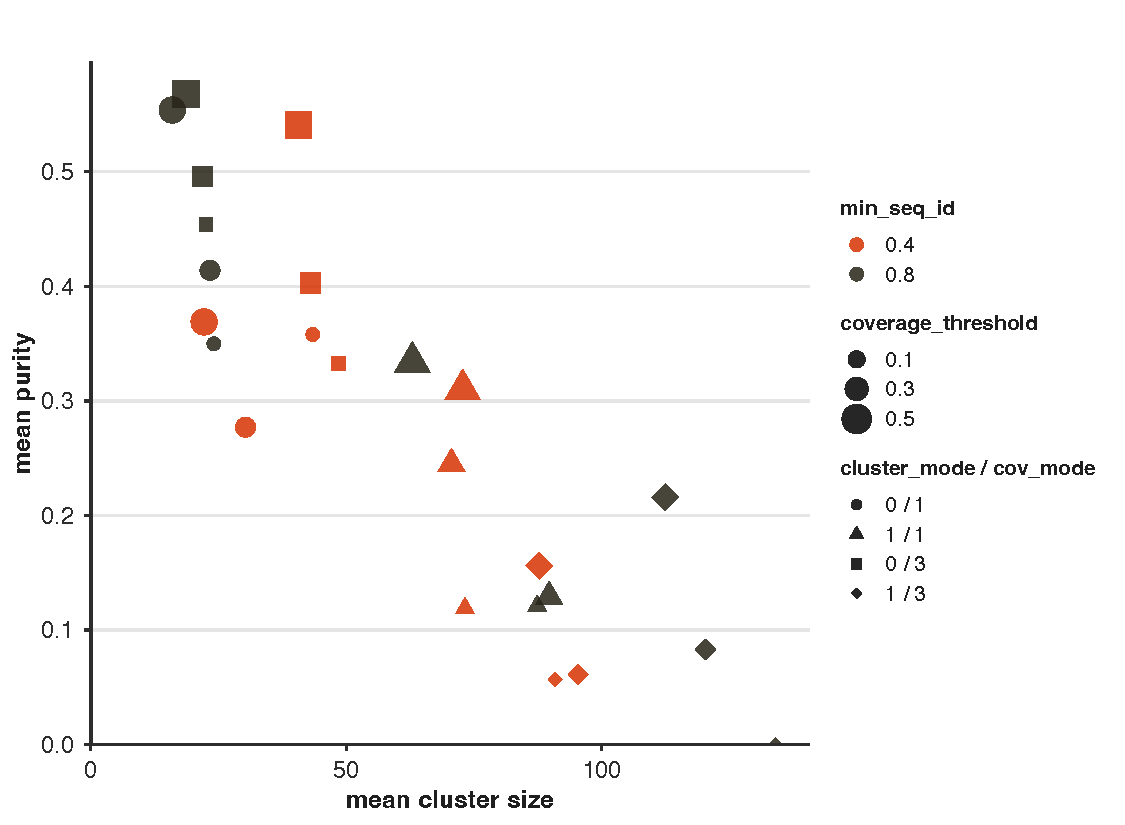
\includegraphics[width=0.95\textwidth]{figures/methods/tradeoff.pdf}
    \caption[Clustering parameter selection for positive control pipeline]{\textbf{Clustering parameter selection for positive control pipeline.}
    The clustering step of the positive control pipeline was run with a range of parameters, and the number of clusters and singleton-genome clusters were recorded.}
    \label{fig:poscontrol-clustering}
\end{figure}

\begin{figure}[H]
  \centering
  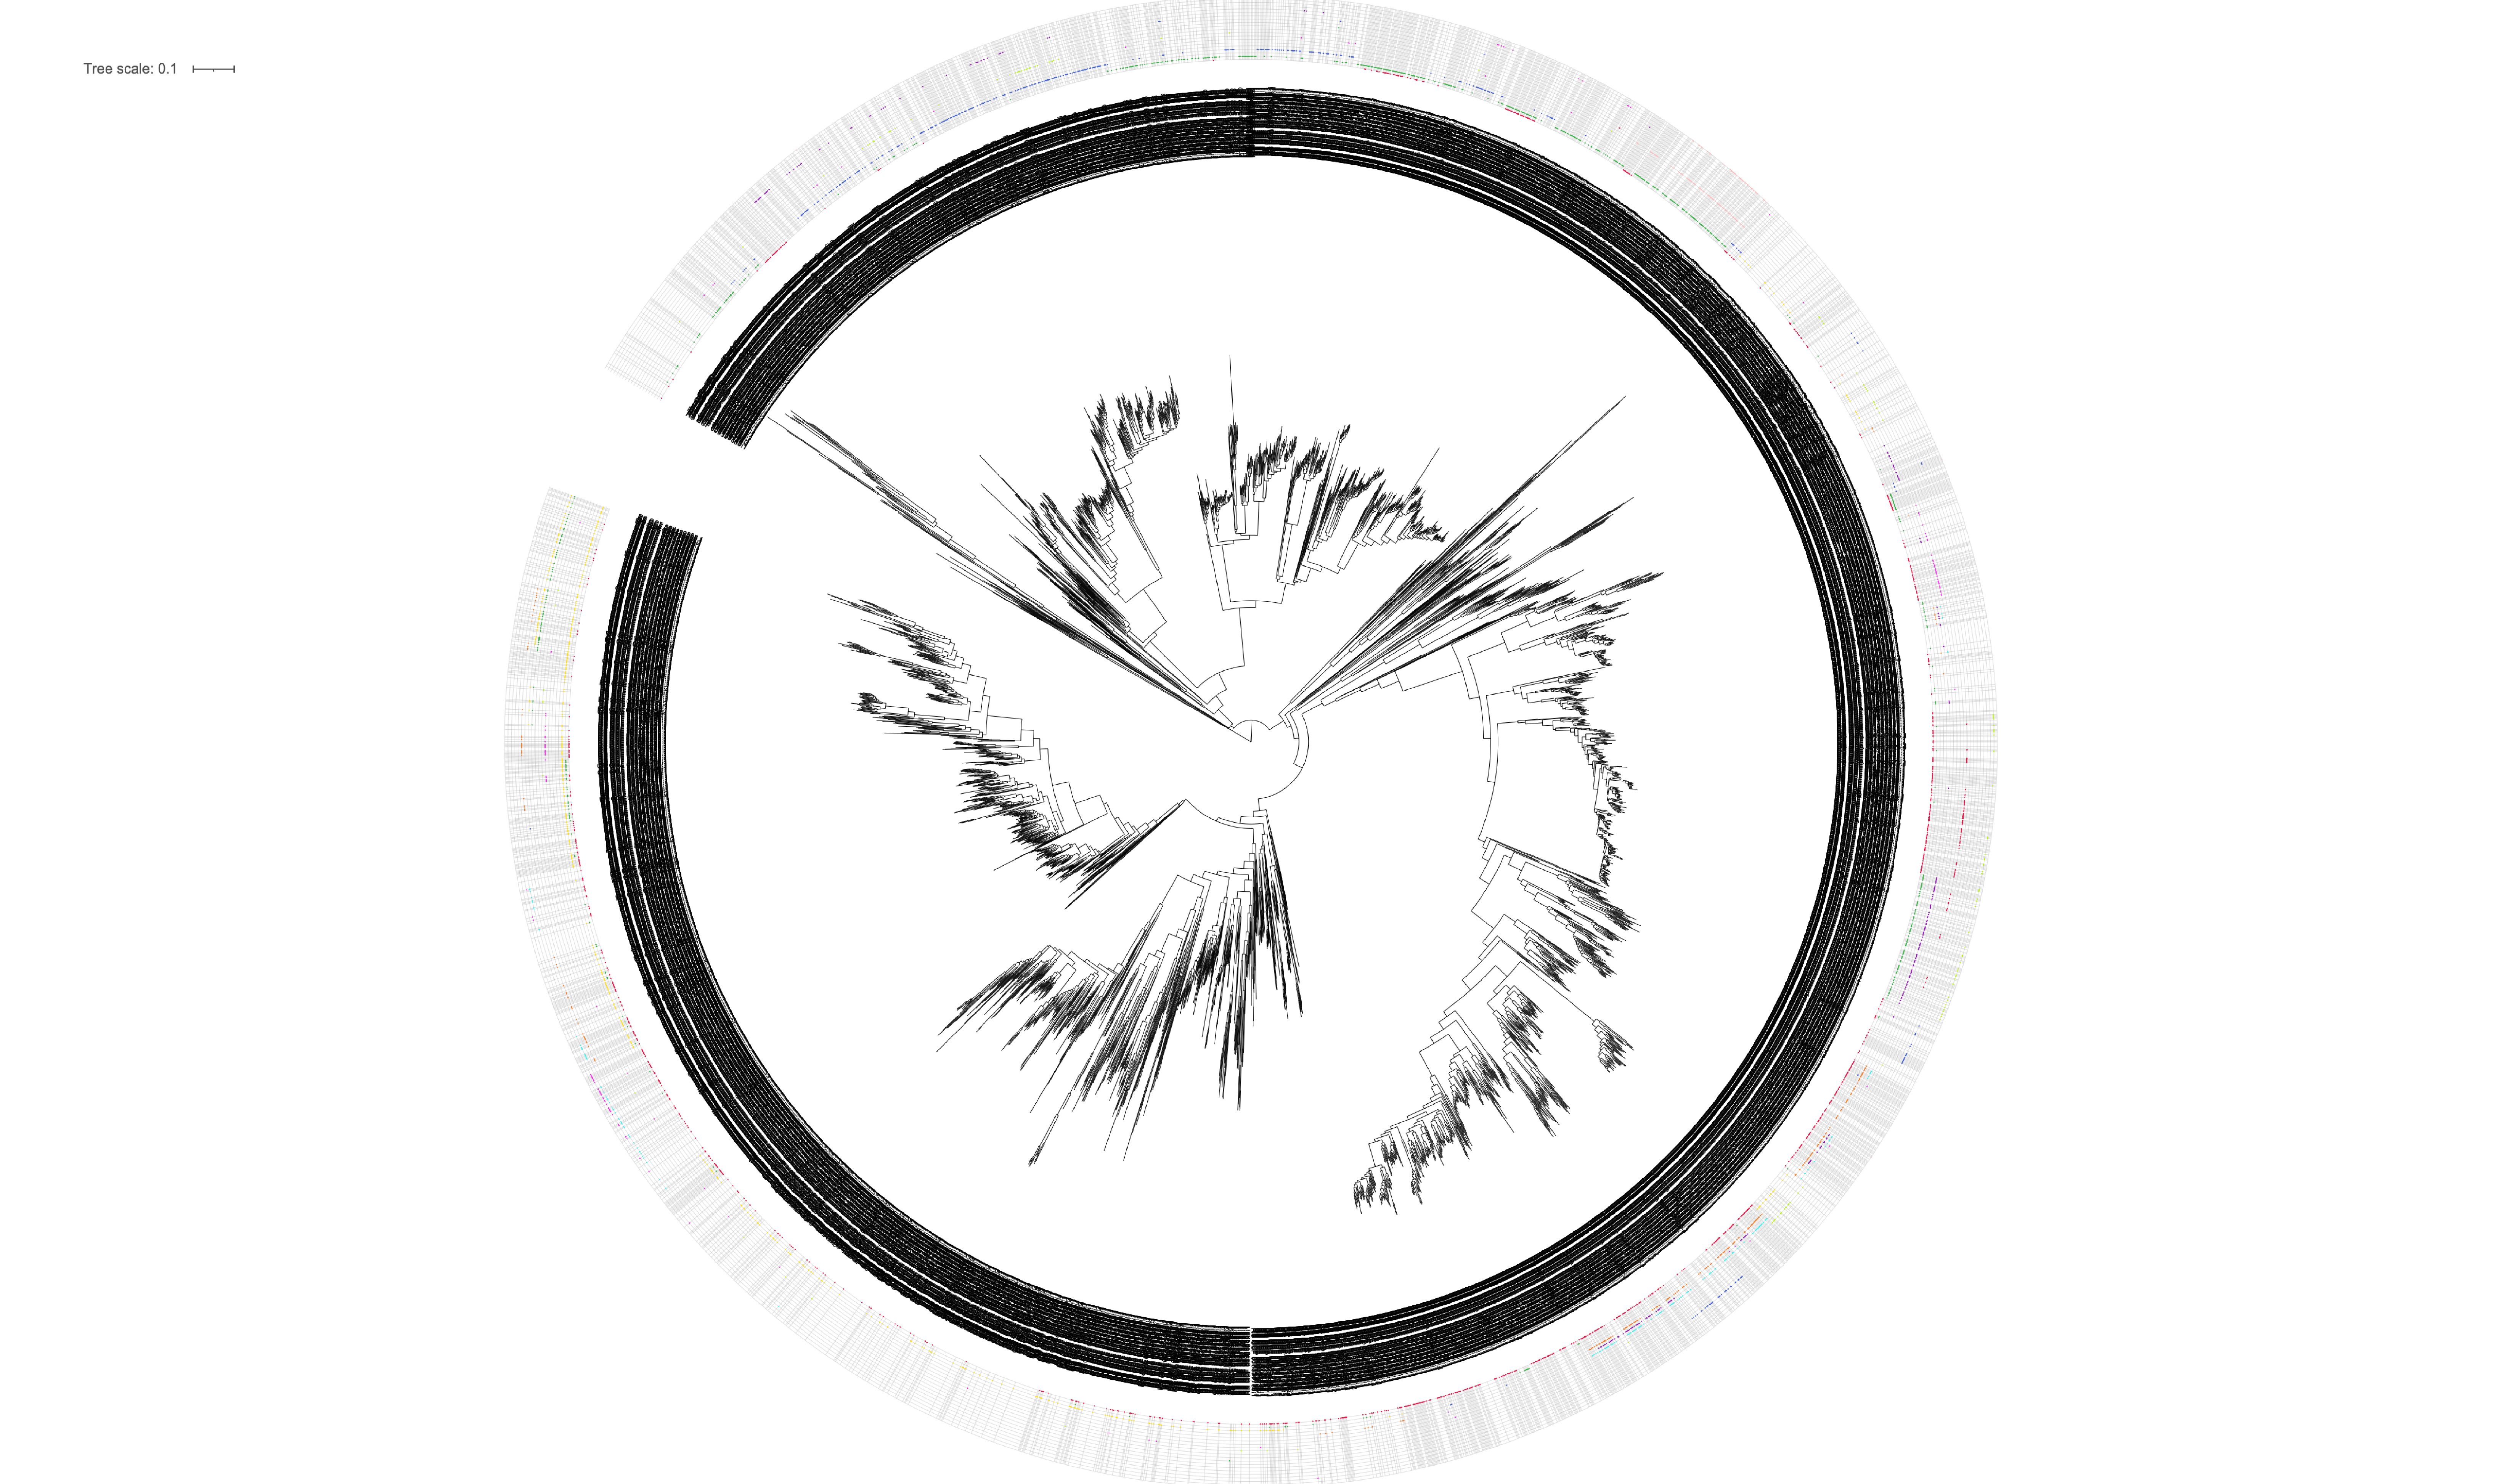
\includegraphics[width=0.95\textwidth]{figures/results/iTOL-gtdbtree-RF00050-clusterannotated.pdf}
  \caption[Prevalence of homologous protein sequences neighbouring \ac{FMN} riboswitch]{\textbf{Prevalence of homologous protein sequences neighbouring \ac{FMN} riboswitch.}
  Top 10 clusters by presence per genome are shown around tree, in order of Appendix Table \ref{tab:cluster_appendix}.
  Tree is annotated with analysis output of the positive control preperation pipeline output.
  It shows the \ac{GTDB} species taxonomy of representative genomes containing the \ac{FMN} riboswitch (as annotated by Rfam).}
  \label{fig:fmn-itol-tree}
\end{figure}

\begin{figure}[H]
  \centering
  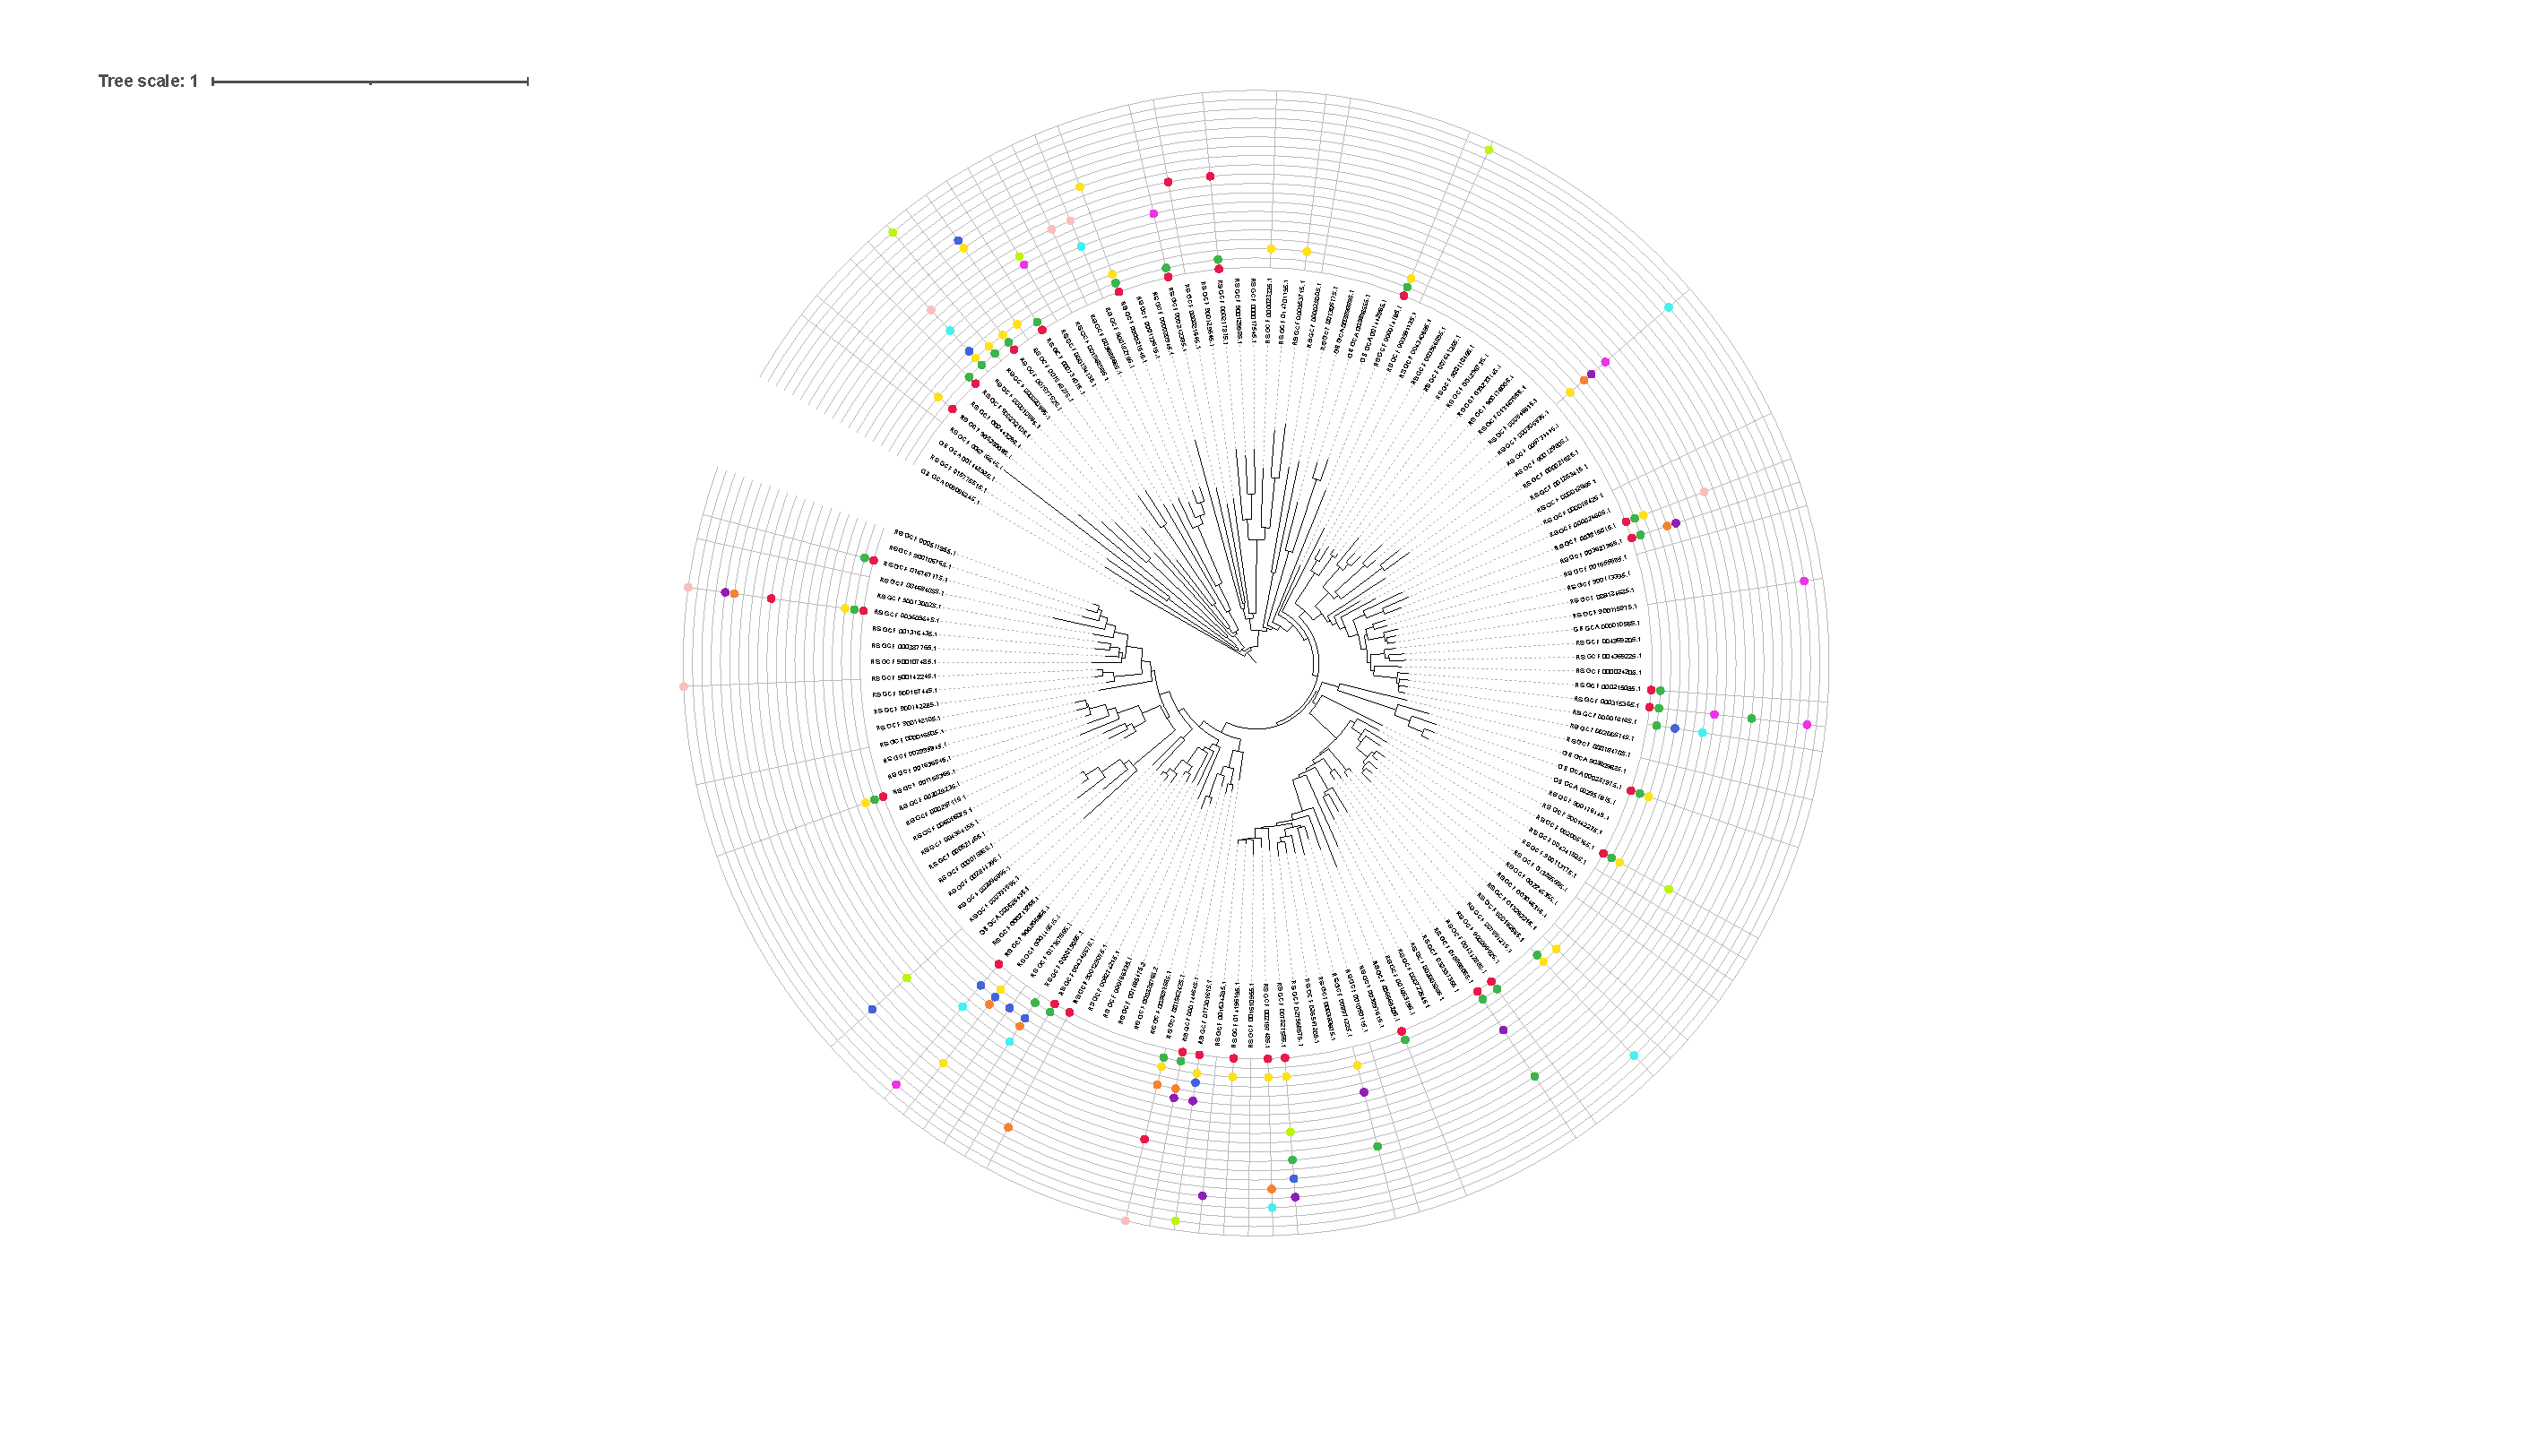
\includegraphics[width=0.95\textwidth]{figures/results/crisprrepeatelementtree.pdf}
  \caption[Prevalence of homologous protein sequences neighbouring \ac{CRISPR}-Direct Repeat 42]{\textbf{Prevalence of homologous protein sequences neighbouring \ac{CRISPR}-Direct Repeat 42.}
  Top 10 clusters by presence per genome are shown around tree, in order of Appendix Table \ref{tab:cluster_appendix}.
  Tree is annotated with analysis output of the positive control preperation pipeline output.
  It shows the \ac{GTDB} species taxonomy of representative genomes containing \ac{CRISPR}-Direct Repeat 42 (as annotated by Rfam).}
  \label{fig:cdr-itol-tree}
\end{figure}

\begin{figure}[p]
    \centering
    \begin{subfigure}[t]{0.48\textwidth}
        \centering
        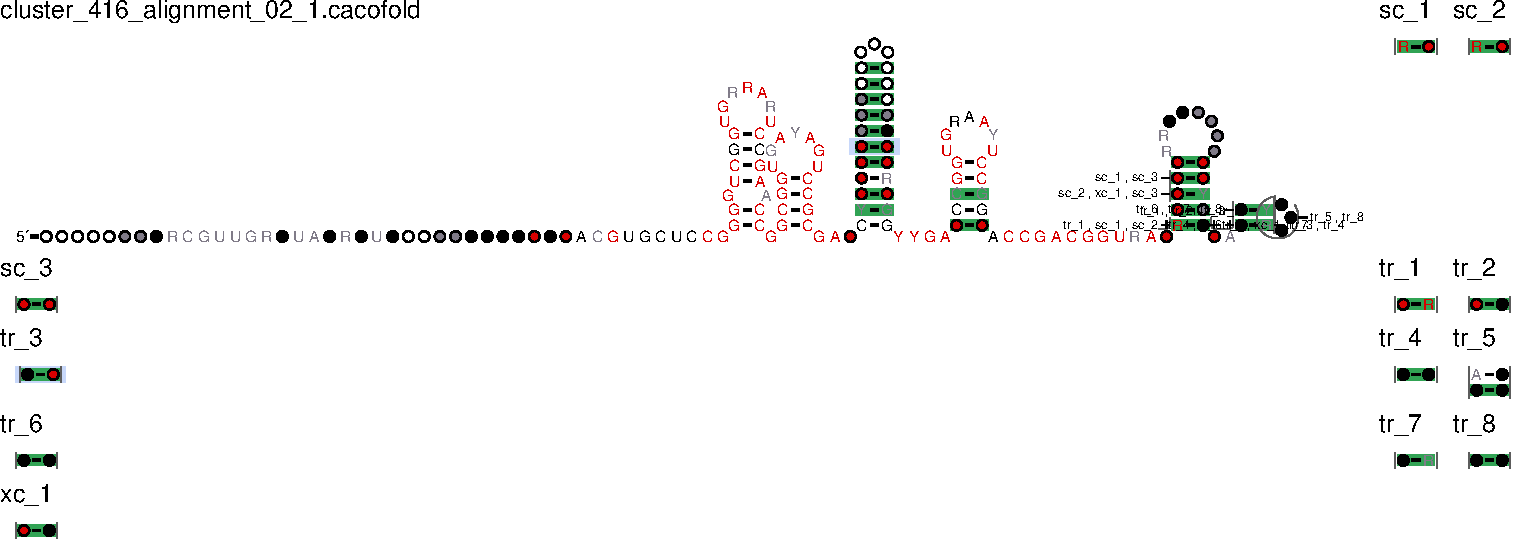
\includegraphics[width=\linewidth]{figures/results/drh-iteritive-expansion-structures/cluster_416_alignment_02_1.cacofold.R2R.sto.pdf}
        \caption{Candidate 416 (F = 78.95)}
        \label{fig:cand416-struct}
    \end{subfigure}
    \hfill
    \begin{subfigure}[t]{0.48\textwidth}
        \centering
        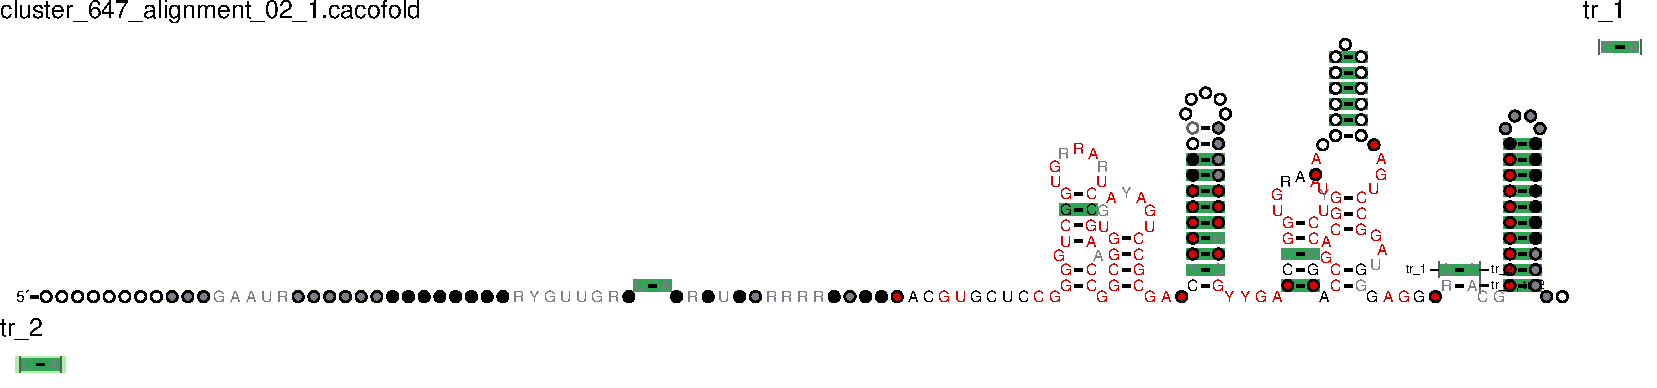
\includegraphics[width=\linewidth]{figures/results/drh-iteritive-expansion-structures/cluster_647_alignment_02_1.cacofold.R2R.sto.pdf}
        \caption{Candidate 647 (F = 73.17)}
        \label{fig:cand647-struct}
    \end{subfigure}

    \vspace{1em}

    \begin{subfigure}[t]{0.48\textwidth}
        \centering
        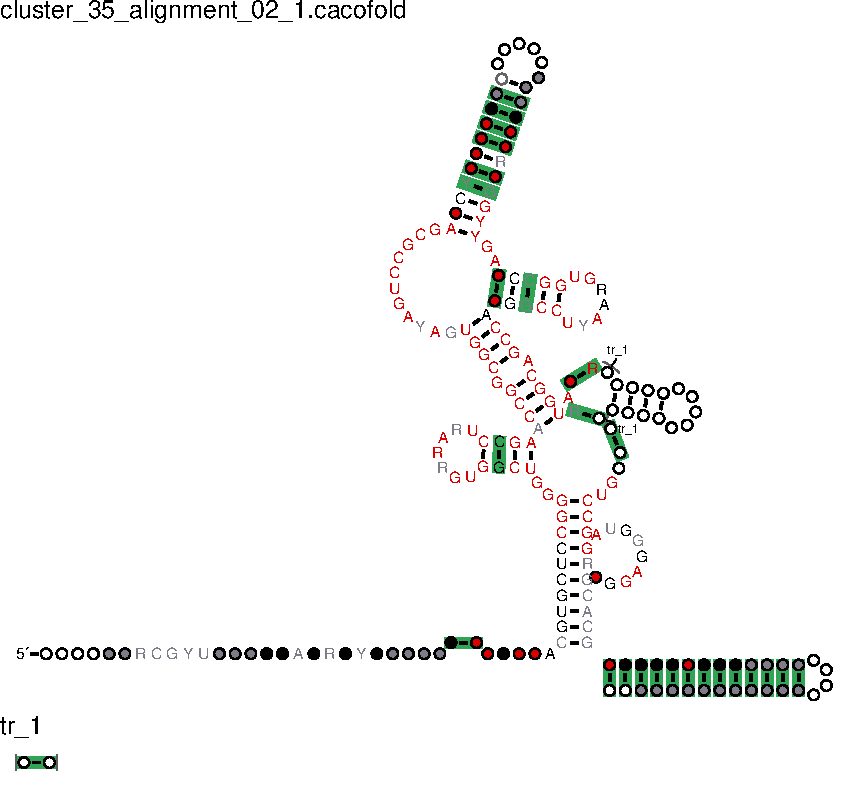
\includegraphics[width=\linewidth]{figures/results/drh-iteritive-expansion-structures/cluster_35_alignment_02_1.cacofold.R2R.sto.pdf}
        \caption{Candidate 35 (F = 62.07)}
        \label{fig:cand35-struct}
    \end{subfigure}
    \hfill
    \begin{subfigure}[t]{0.48\textwidth}
        \centering
        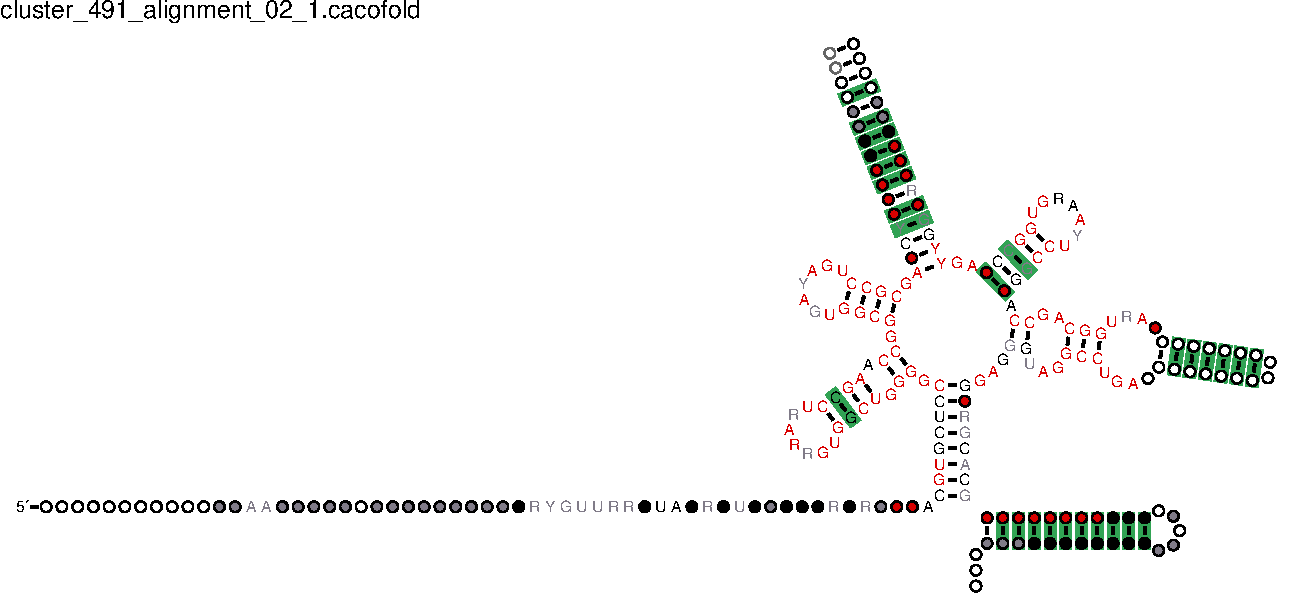
\includegraphics[width=\linewidth]{figures/results/drh-iteritive-expansion-structures/cluster_491_alignment_02_1.cacofold.R2R.sto.pdf}
        \caption{Candidate 491 (F = 60.67)}
        \label{fig:cand491-struct}
    \end{subfigure}

    \vspace{1em}

    \begin{subfigure}[t]{0.48\textwidth}
        \centering
        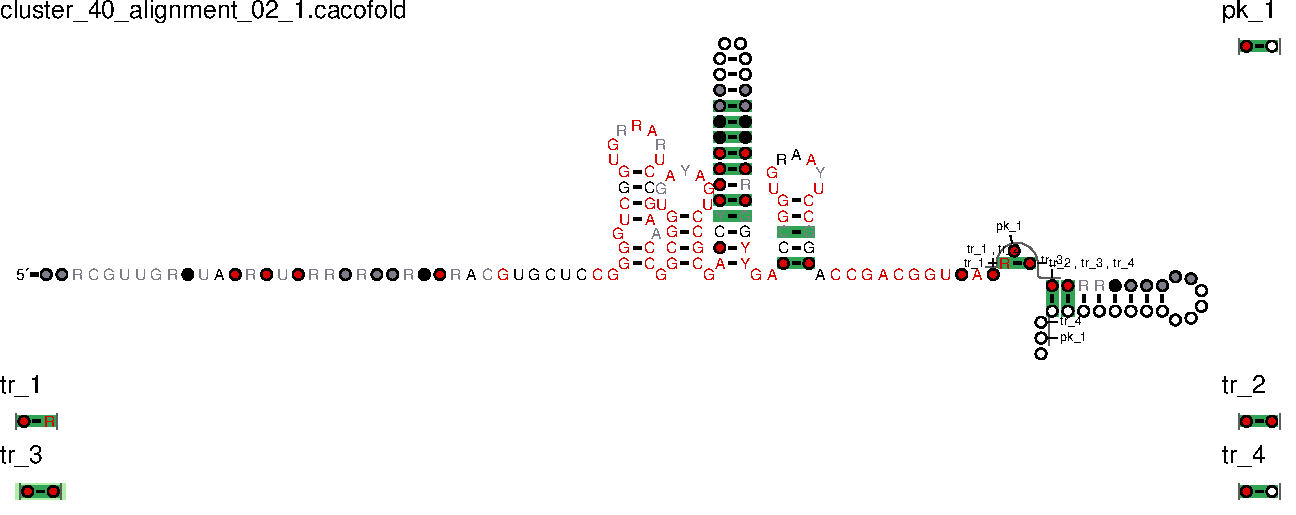
\includegraphics[width=\linewidth]{figures/results/drh-iteritive-expansion-structures/cluster_40_alignment_02_1.cacofold.R2R.sto.pdf}
        \caption{Candidate 40 (F = 56.67)}
        \label{fig:cand40-struct}
    \end{subfigure}

    \caption[Predicted covarying secondary structures of remaining FMN candidates, part 1]{\textbf{Predicted covarying secondary structures of remaining FMN riboswitch candidates (part 1 of 2).} R-scape CaCoFold structures generated from iteratively expanded alignments, ordered by F-score.}
    \label{fig:drh-appendix-structures-1}
\end{figure}

\begin{figure}[p]
    \centering
    \begin{subfigure}[t]{0.48\textwidth}
        \centering
        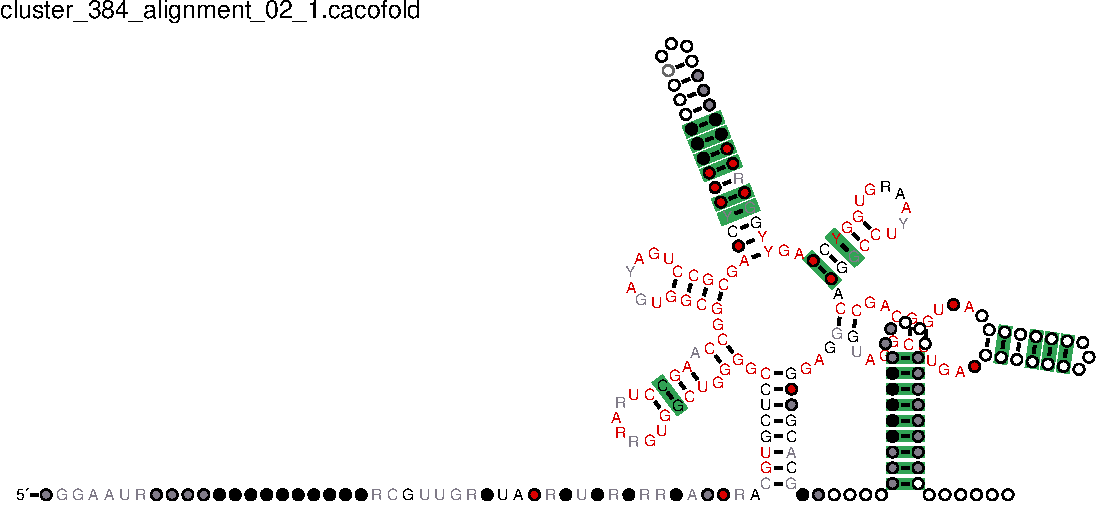
\includegraphics[width=\linewidth]{figures/results/drh-iteritive-expansion-structures/cluster_384_alignment_02_1.cacofold.R2R.sto.pdf}
        \caption{Candidate 384 (F = 55.70)}
        \label{fig:cand384-struct}
    \end{subfigure}
    \hfill
    \begin{subfigure}[t]{0.48\textwidth}
        \centering
        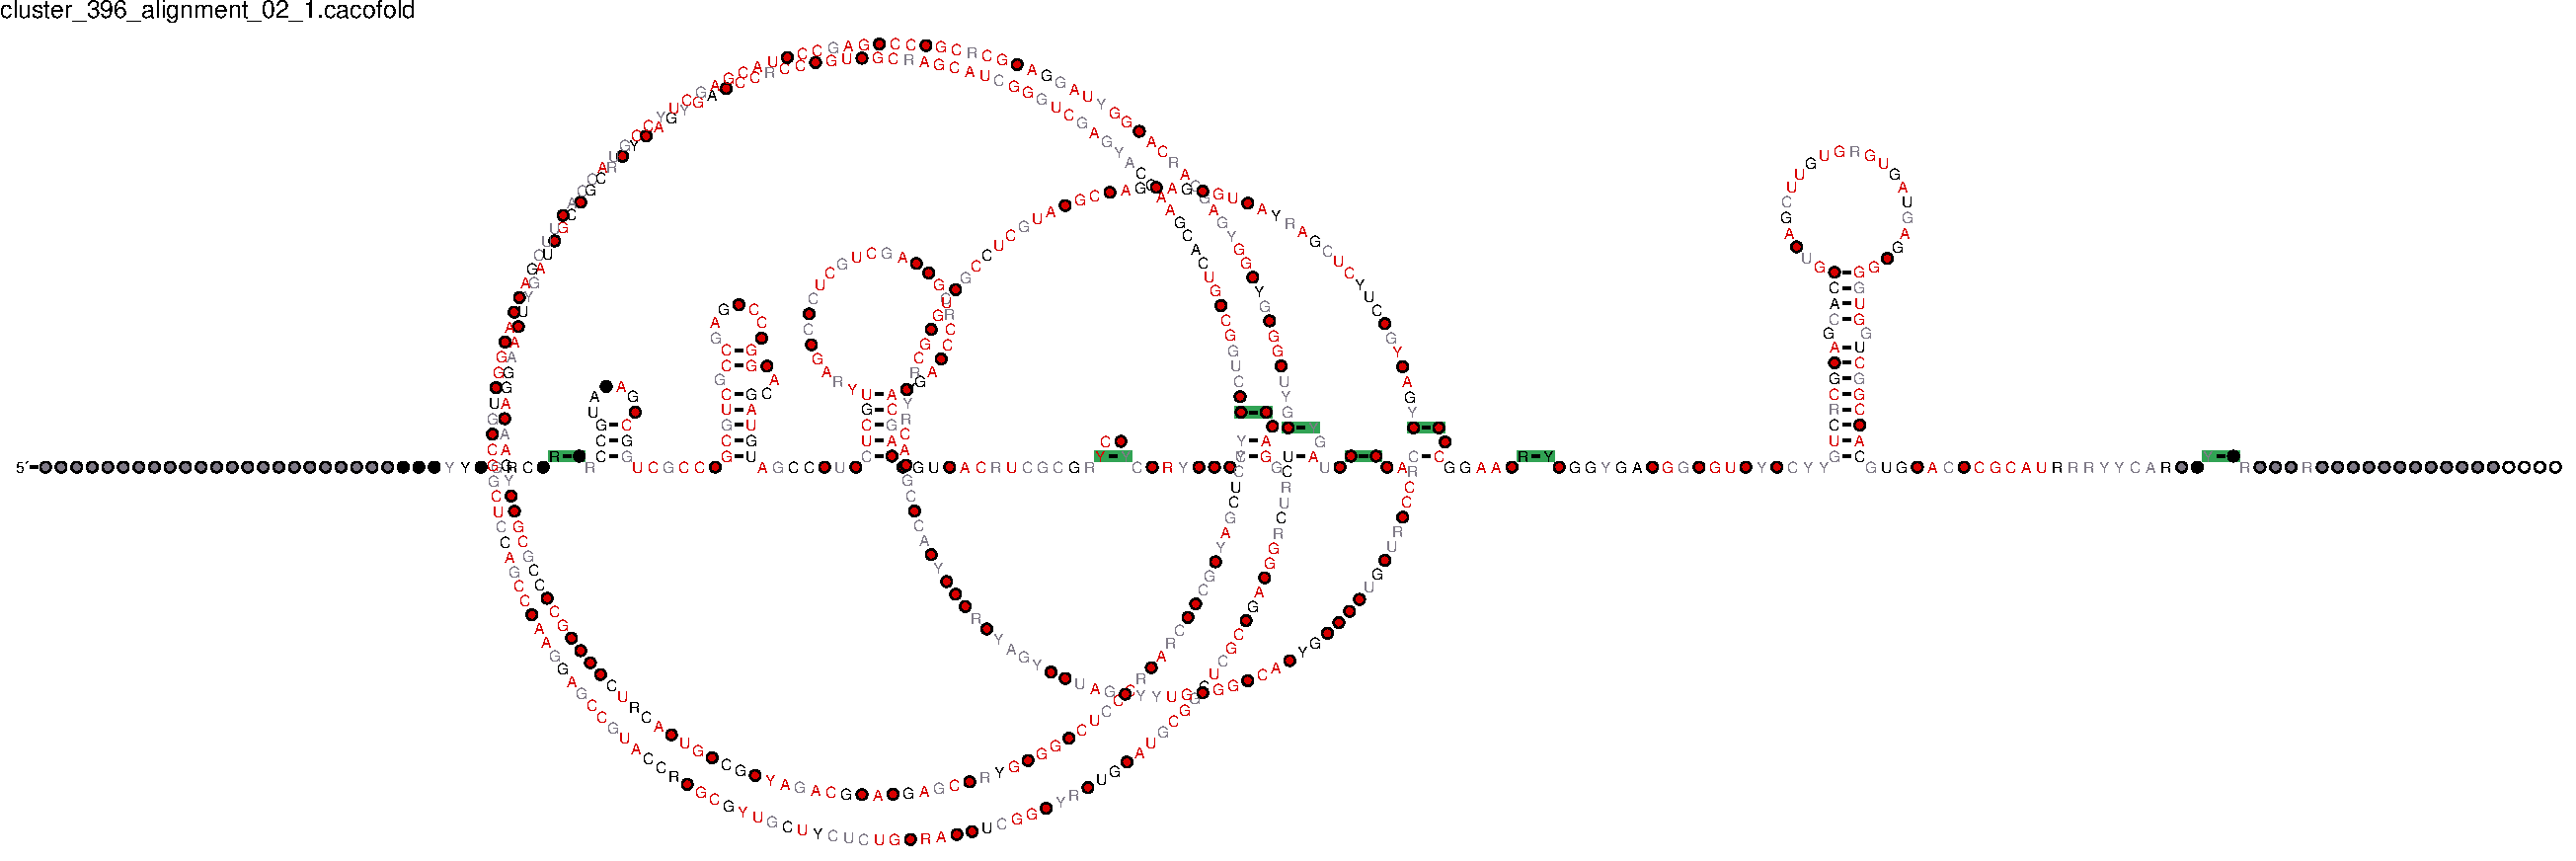
\includegraphics[width=\linewidth]{figures/results/drh-iteritive-expansion-structures/cluster_396_alignment_02_1.cacofold.R2R.sto.pdf}
        \caption{Candidate 396 (F = 34.04)}
        \label{fig:cand396-struct}
    \end{subfigure}

    \vspace{1em}

    \begin{subfigure}[t]{0.48\textwidth}
        \centering
        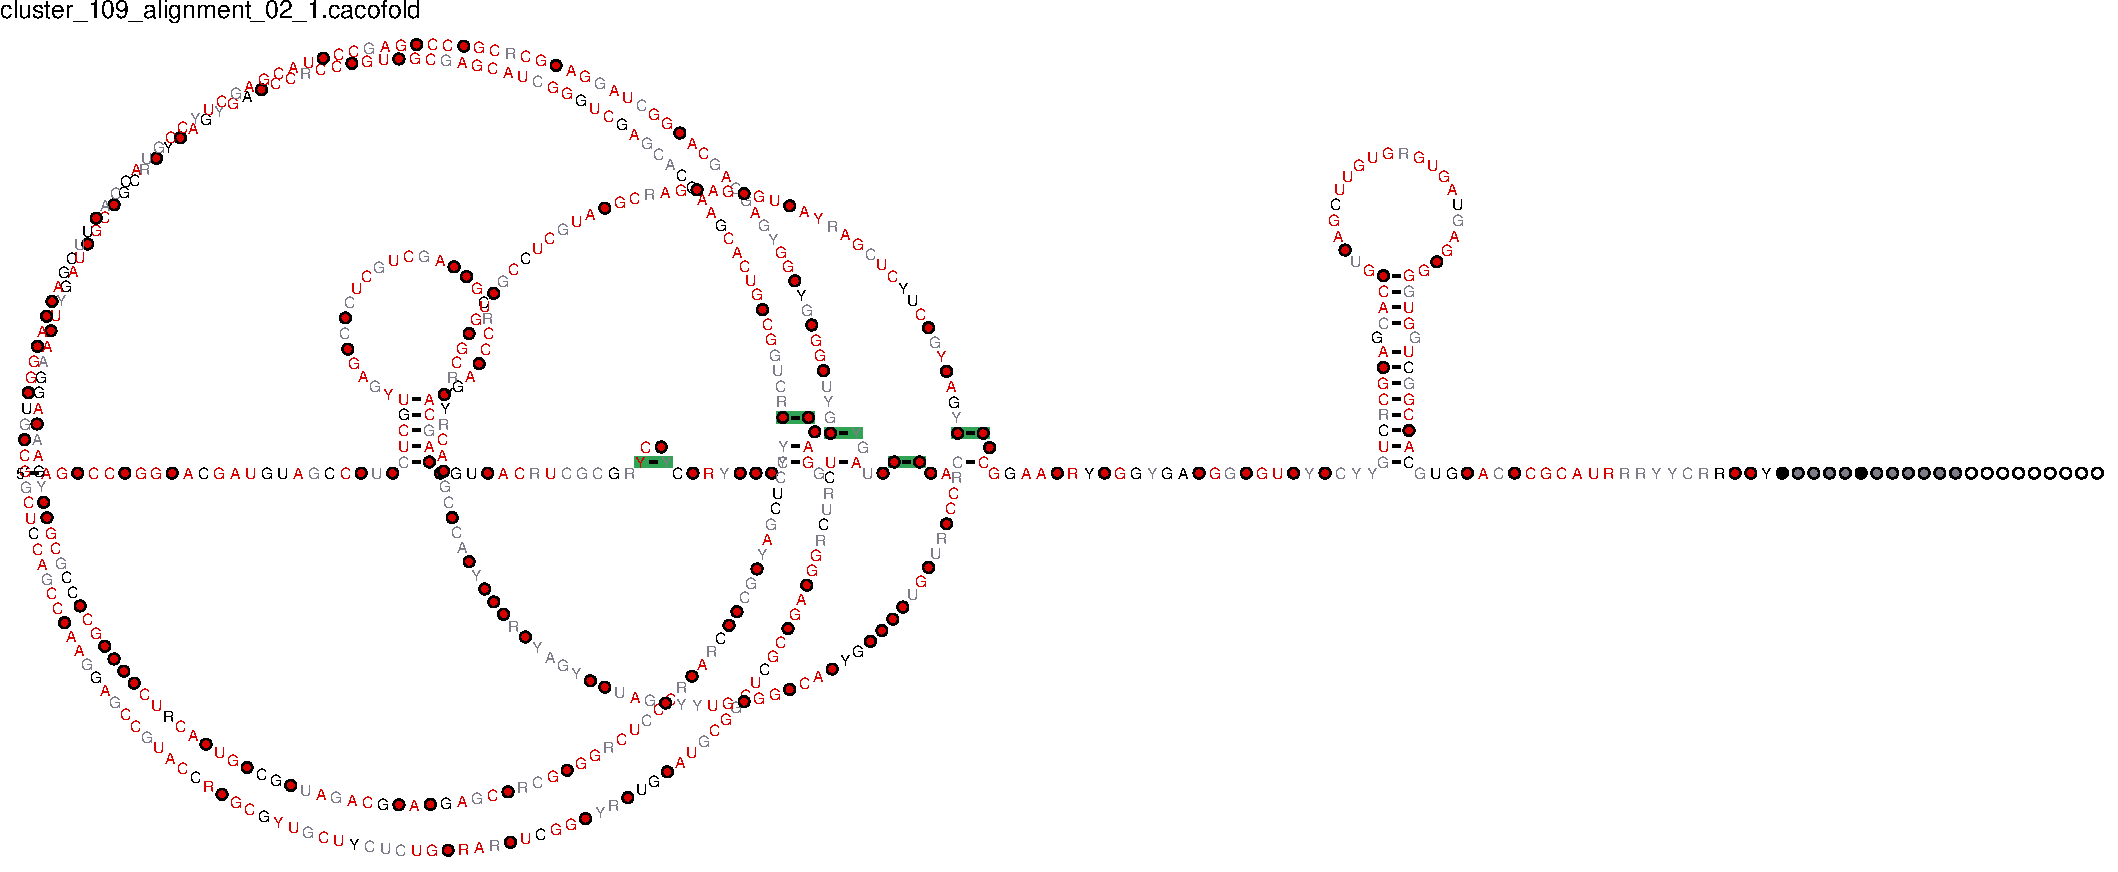
\includegraphics[width=\linewidth]{figures/results/drh-iteritive-expansion-structures/cluster_109_alignment_02_1.cacofold.R2R.sto.pdf}
        \caption{Candidate 109 (F = 32.26)}
        \label{fig:cand109-struct}
    \end{subfigure}
    \hfill
    \begin{subfigure}[t]{0.48\textwidth}
        \centering
        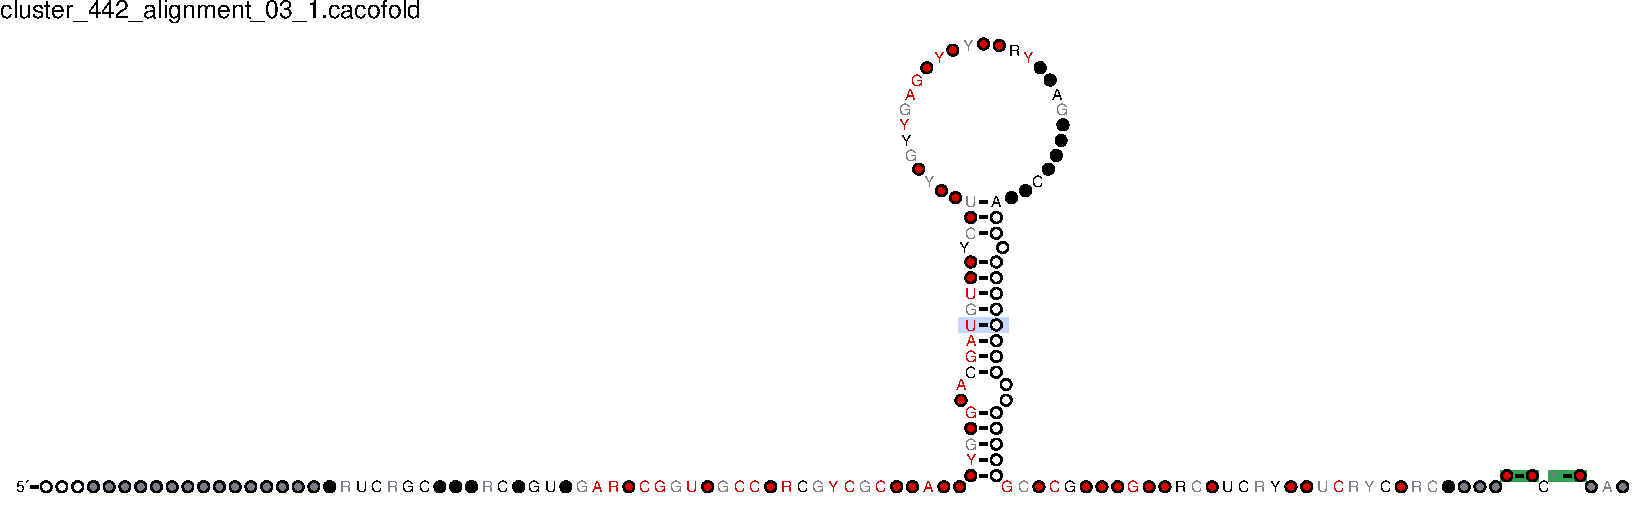
\includegraphics[width=\linewidth]{figures/results/drh-iteritive-expansion-structures/cluster_442_alignment_03_1.cacofold.R2R.sto.pdf}
        \caption{Candidate 442 (F = 20.00)}
        \label{fig:cand442-struct}
    \end{subfigure}

    \caption[Predicted covarying secondary structures of remaining FMN candidates, part 2]{\textbf{Predicted covarying secondary structures of remaining FMN riboswitch candidates (part 2 of 2).} R-scape CaCoFold structures generated from iteratively expanded alignments, ordered by F-score. \ref{fig:cand396-struct} and \ref{fig:cand109-struct} correspond to the two low-identity outlier clusters discussed in the results text.}
    \label{fig:drh-appendix-structures-2}
\end{figure}
\clearpage

\begin{figure}[H]
    \centering
    \begin{subfigure}[t]{0.48\textwidth}
        \centering
        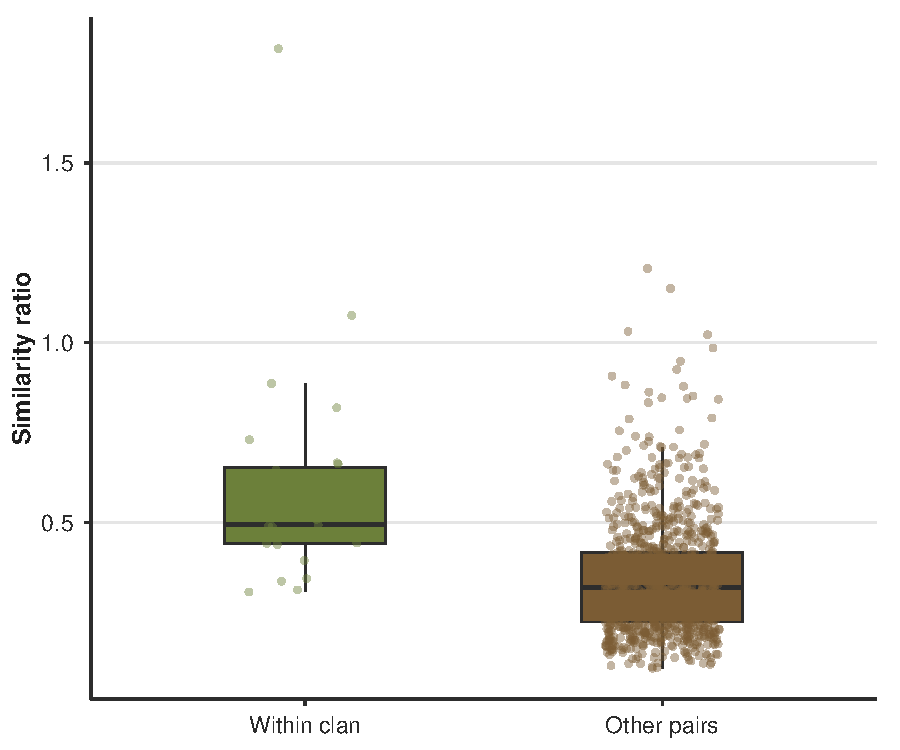
\includegraphics[width=\linewidth]{figures/results/cm-simile/similarity_ratio_boxplot.pdf}
        \caption{Similarity ratio (minmax)}
        \label{fig:similarity-ratio-boxplot}
    \end{subfigure}
    \hfill
    \begin{subfigure}[t]{0.48\textwidth}
        \centering
        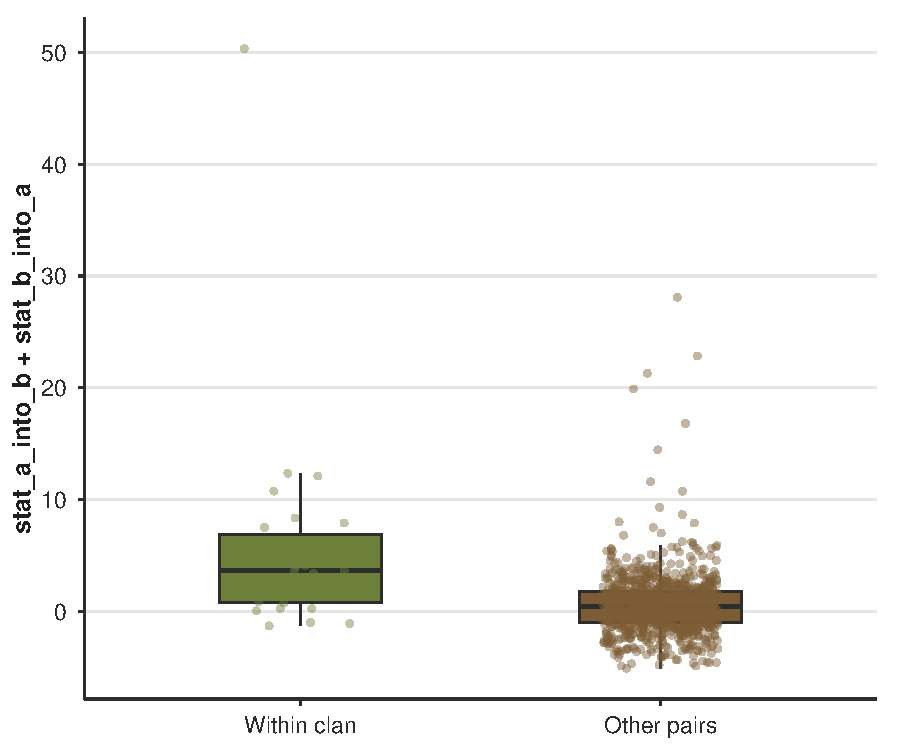
\includegraphics[width=\linewidth]{figures/results/cm-simile/bitscoresumdifference_boxplot.pdf}
        \caption{Bitscore median vs.\ null}
        \label{fig:bitscore-boxplot}
    \end{subfigure}
    \caption[Within- vs.\ between-clan separation for early classification approaches]{\textbf{Within- vs.\ between-clan separation for the two initial classification approaches.} 
    \textbf{(a)}: shows pairwise similarity ratio scores, motivated by common-ancestor theory but lacking a statistical null. 
    \textbf{(b)}: shows median bitscore compared against a dinucleotide-shuffled bootstrap null distribution. 
    Within-clan (\emph{n}~=~27) and other (\emph{n}~=~919) pairs are drawn from annotated Rfam entries.}
    \label{fig:early-classifiers}
\end{figure}